\section{Struttura della comunicazione fra le entità} 
La Figura \ref{fig:covertchannel:struttura:flow} mostra il flusso di 
comunicazione fra le entità coinvolte nella comunicazione covert channel. 
Di seguito la descrizione di ciascuna entità. 
\begin{itemize}
    \item \textbf{Attaccante}: \newline 
    Carica un file di configurazione nel quale viene definito l'indirizzo IP della vittima, 
    il metodo di attacco e i proxy utilizzabili per farlo. 
    Inoltre inserirà il comando che la vittima dovrà eseguire o il dato che gli si vuole mandare. 
    Nel caso utilizzasse dei proxy, aspettera da essi i dati che la vittima restituirà. 
    \item \textbf{Proxy}: \newline 
    Ha bisongo di sapere l'indirizzo IP dell'attaccante siccome deve ottenre 
    da esso l'indirizzo IP della vittima e il comando da inoltrarle. 
    Una volta stabilita una connessione sia con l'attaccante che con la vittima; 
    si occuperà di inoltrare i dati che le due entità si scambiano. 
    \item \textbf{Vittima}: \newline 
    Aspetta le connessioni o dall'attaccante o dai proxy (se vengono utilizzati). 
    Rimane in attesa di un comando (o di un dato). 
    Nel primo caso lo eseguirà e successivamnete invierà i dati ricavati. 
\end{itemize} 
\vspace{3ex} 
\begin{center} 
    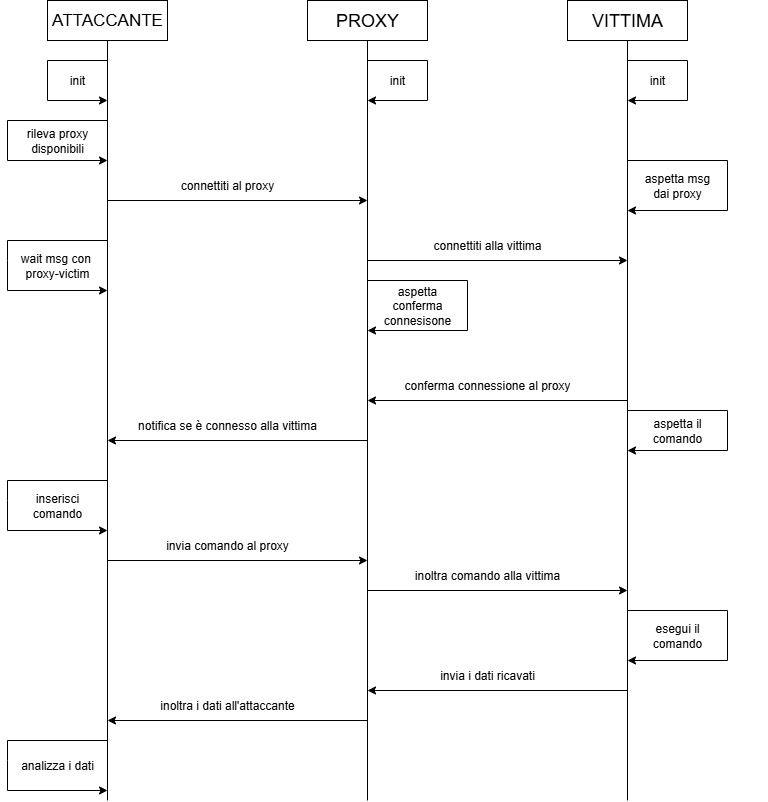
\includegraphics[width=\textwidth]{../img/implementazione/diagramma_struttura_entita.jpg} 
\captionof{figure}{Flusso di comunicazione fra le entita \cite{draw_io}} 
    \label{fig:covertchannel:struttura:flow} 
\end{center}  
Il canale di comunicazione che il proxy e l'attaccante potranno avere 
dipende dall'affidabilità di quest'ultimo\footnote{
    Durante lo sviluppo si sono ritenuti i proxy affidabili
}: 
\begin{itemize} 
    \item Nel caso si reputi il proxy insicuro, si potrà utilizare una 
    comunicazione TCP così da avere una comunicazione stabile e affidabile. 
    \item Se invece si reputa il proxy non non sicuro (e quindi si dovrà 
    nascondere la comunicazione anche da lui), si potrà usare la comunicazione usata con la vitima. 
    Quindi il proxy e l'attacante comunicheranno tramite pachetti ICMP.
    Questa tipologia di comunicazione è più instabile rispetto alla precedente 
    ma garantisce un maggior anonimato. 
\end{itemize}  
Riguardo la comunicazione; l'attaccante potrà usare uno (il caso standard) 
o più proxy per comunicare con la vittima (come mostrato nella Figura \ref{fig:covertchannel:struttura:schema}). 
Tuttavia sarà anche possibile (per l'attaccante) anche comunicare direttamente con la vittima.  
In questo caso alcune funzioni presenti nel proxy verranno eseguite dall'attaccante 
(e.g connettersi alla vittima). 
Mentre nel precedente invece, si deve prevedere un metodo per poter riordinare i 
messaggi che l'attaccante ha ricevuto dai proxy\footnote{
    Ciò è stato fatto inserendo un indice al pacchetto inviato dal proxy
}. 
\vspace{3ex}\newline
\begin{center} 
    \captionof{figure}{Struttura e dialogo delle entità presenti \cite{draw_io}}
    \label{fig:covertchannel:struttura:schema} 
    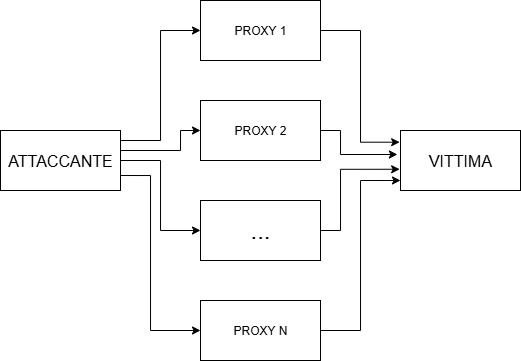
\includegraphics[width=0.7\textwidth]{../img/implementazione/struttura attacker.proxy.victim 3.jpg} 
\end{center} 

\subsection{Struttura dell'attaccante}  
Tramite un parser rileve se nella linea di comando sono state inserite le opzioni 
descritte nella Tabella \ref{table:comunicazione:attacccante:opzioni}.
Queste sono necessarie alla sua inizializzazione. 
\begin{longtable}{|p{0.3\textwidth}|p{0.6\textwidth}|} 
\caption{Opzioni richieste nel comando dell'attaccante} 
\label{table:comunicazione:attacccante:opzioni} \\
    \hline 
    \textbf{Opzione} & \textbf{Utilizzo}  \\
    \hline
    Path file & 
    Percorso per il file di configuraizone da caricare. In questo file JSON viene specificato 
    l'indirizzo IP della vittima, la metodologia di attacco e la lista dei proxy che si vogliono usare. 
    \\ 
    \hline  
\end{longtable} 
\vspace{2ex} 
Per ogni proxy specificato nel file di configurazione, si verifica quali sono disponibili; 
ovvero quali proxy sono connessi sia all'attaccante che alla vititma.  
Per farlo si crea un canale di comunicazione con ciascun proxy, o tramite ICMP o TCP/IP, 
e si invia un messaggio di connessione. 
In questo messaggio si specifica sia l'indirizzo IP della vittima che la metodologia di attacco scelta.
Successivamente si rimarrà in attesa che il proxy confermi la connessione con la vittima.  
\vspace{2ex} \newline 
Nel caso non si usassero dei sockets TCP/IP ma il protocollo ICMP, bisognerà definire un thread 
che si occupi di monitorare il traffico di rete per poter catturare i messaggi ICMP contenenti i dati 
inviati dai proxy. 
Quindi prima di inviare alcun comando (o dato), bisogna assicurarsi che il thread sia già partito altrimenti si 
potrebbero perdere delle informazioni. 
\vspace{1ex} \newline
Una volta ricevuti tutti i dati inoltrati dai proxy, l'attaccante dovrà riordinarli per ricavare il messaggio. 
Inoltre se si volesse mandare un altro comando, si dovranno reimpostare le variabili necessarie per farlo.
Altrimenti si può decidere di interrompere la comunicazione e in quel caso i proxy ne verranno aggiornati. 


\subsection{Struttura del Proxy} 
Come per l'attaccante, anche il proxy necessita di alcune opzioni (descritte nella Tabella \ref{table:comunicazione:proxy:opzioni}). 
\newline
\begin{minipage}{\textwidth}
\begin{longtable}{|p{0.3\textwidth}|p{0.6\textwidth}|} 
\caption{Opzioni richieste nel comando del proxy} 
\label{table:comunicazione:proxy:opzioni} \\
    \hline 
    \textbf{Opzione} & \textbf{Utilizzo}  \\
    \hline
    Indirizzo IP & 
    Rappresenta l'indirizzo IP dell'attaccante. Quando il proxy crea il socket e rimane in ascolto delle connessioni, 
    accetterà solo quelle che combaciano con questo indirizzo; qualunque altra connessione verrà rifiutata. 
    Questo viene fatto anche nel caso di un canale tramite ICMP. 
    \\ 
    \hline 
\end{longtable} 
\end{minipage}
\vspace{2ex}  \newline 
Per poter comunicare con l'attaccante, il proxy definisce un socket in cui rimane in ascolto. 
Nel caso si utilizzi il protoccollo ICMP, monitorerà il flusso di rete per catturare i messaggi inviati dall'attaccante. 
Stabilita una comunicazione con esso, il proxy aspetterà un messaggio indicante l'indirizzo IP della 
vittima oltre alla tipologia di Covert Channel scelto. 
\vspace{1ex} \newline 
I messaggi che un proxy può ricevere dall'attacante sono: 
\begin{enumerate} 
    \item Il messaggio indicante il comando (che il proxy dovrà inoltrare 
    alla vittima) oppure se deve aspettare solo i dati 
    (siccome non ha ricevuto il comando). 
    \item Il messaggio che indica la terminazione della comunicazione con l'attacante. 
    In questo caso il proxy aggiornerà la vittima della cosa. 
\end{enumerate} 
Per la connessione con la vittima, il proxy comunicherà tramite pacchetti ICMP. 
Prima di inviare alcun dato, si imposta un thread con lo scopo di analizzare il traffico e catturare i dati che 
la vittima ritornerà.  
Se questo viene fatto dopo i pacchetti potrebbero andare persi.  
Una volta ricevuti tutti i dati dalla vittima, il proxy procederà ad inoltrarli all'attaccante.  

\subsection{Struttura Vittima} 
Per poterla inizializzare, la vittima richiede in input alcune opzioni
(indicate nella Tabella \ref{table:comunicazione:vittima:opzioni}). 
\begin{longtable}{|p{0.3\textwidth}|p{0.6\textwidth}|} 
\caption{Opzioni richieste nel comando della vittima} 
\label{table:comunicazione:vittima:opzioni} \\
    \hline 
    \textbf{Opzione} & \textbf{Utilizzo}  \\
    \hline 
    Numero di Proxy & 
    Quando si eseguirà il programma, dovranno essere definiti il numero di proxy necessari. 
    Ciò indicherà il numero minimo di proxy necessari che serviranno per l'esecuzione dell'attacco. 
    Una volta raggiunto questo numero, la vittima procederà con l'esecuzione del comando. 
    Altrimenti, se il numero non viene raggiunto, allo scadere del timer si chiederà se si vuole procedere comunque. 
    \\ 
    \hline  
\end{longtable} 
La vittima rimane in attesa di connessioni da parte dei proxy.
Ciò viene fatto monitornado il flusso di rete e filtrando i messaggi ICMP 
(destinati alla vittima) che rappresentano una richiesta di connessione. 
Se il messaggio ricevuto risulta valido, si invia al mittente un messaggio 
di conferma e il suo l'indirizzo IP viene inserito nella lista indicante i proxy connessi.
Da questo messaggio la vittima ricaverà anche la metodologia di attacco scelto. 
E quindi ciascun proxy potrà usare (se voluto) una diversa tipologia di attacco. 
\vspace{1ex} \newline 
Definiti i proxy con cui si comunicherà, si attenderà che inoltrino il comando dell'attaccante. 
Una volta ricevuto, verrà eseguito e i risultati ricavati (sia quelli legati all'output che quelli legati ad 
eventuali errori) vengono inviati all'attaccante tramite i proxy disponibili. 
Nel caso siano presenti molteplici proxy connessi, si definirà una lista indicante i dati che ciascuno di essi dovrà ricevere. 
L'ultimo messaggio che verrà inviato a ciascuno dei proxy sarà quello che indica che tutti i dati sono stati mandati. 
